\chapter{Data verwerking} \label{ch:dataverwerking}
% inleiding van dit hoofdstuk, wat ga ik allemaal bespreken
% bespreken benodigdheden duidelijke resultaten
In dit hoofdstuk wordt de data verkregen uit vorig hoofdstuk verwerkt in visuele resultaten. De verschillende ondernomen stappen worden besproken. De eerste stap behandelt het verwerpen van bepaalde datapunten. Vervolgens wordt de data met bepaalde parameters in verband gebracht. Tot slot wordt de data op vlak van spreiding geanalyseerd en uiteindelijk in grafiekvorm weergegeven. De resultaten zelf worden in hoofdstuk \ref{ch:resultaten} besproken. 

\section{Data cleaning}
Een belangrijk gebeuren voor de data verwerkt kan worden, is het schoonmaken van de data. Tijdens het uitvoeren van metingen is het mogelijk dat er meetfouten plaatsvinden. Deze kunnen door allerlei oorzaken plaats vinden en moeten zo veel mogelijk vermeden worden. In deze sectie bespreken we een aantal van deze meetfouten en hoe deze aangepakt en verwerkt worden. 
% verwerpen van data in vorig hoofdstuk,
% voorbeeld van verworpen data weergeven.
% deel dat al in data verwerving is gebeurd(selectie data)
	\subsection{Verwerpen data}
	Een eerste wijze van schoonmaken is het verwerpen van datapunten waarvan er geweten is dat deze onmogelijk correct kunnen zijn. Dit betreft meetfouten waar bijvoorbeeld de duur van het uitvoeren van een programma gelijk is aan nul seconden. Dit is uiteraard niet mogelijk, elke meting heeft namelijk een duur van een bepaalde grootte. Een andere meetfout die geregeld op trad kwam bij het meten van het \gls{cpu}-verbruik voor. Indien na het uitvoeren van een programma bleek dat er geen activiteit in de \gls{cpu} werd gemeten is dit als gevolg van een meetfout. 
	
	Indien deze meetfouten worden gedetecteerd zal de volledige meting worden verworpen en wordt de meting herhaald. De controle op deze meetfouten vindt dus plaats na het uitvoeren van de meting en voor het opslaan van de data. In listing \ref{lst:meetfout} kan deze controle teruggevonden worden. Alleen nadat er geen meetfout gedetecteerd wordt de data uitgeschreven en wordt de iteratie erkend als een geldige iteratie. Door een imperfecte meting te hernemen blijft het totaal aantal bruikbare datapunten bijgevolg altijd 20.
	
	\newpage
	
	\begin{lstlisting}[caption={Controleren op meetfouten.}, captionpos=b,label={lst:meetfout}]
# Meting wordt gecontroleerd voor 
if (mean(cores) != 0.0) and (time_stop-time_start != 0):
	logging_data(10, time_stop, time_start, cores)
	iteration += 1
print("iteration: ", iteration, " mean cores: ", mean(cores), " duration: ", time_stop-time_start)
\end{lstlisting}
	
	
	\subsection{Behandelen uitschieters}
	De tweede wijze waarop de data wordt schoon gemaakt is door het behandelen van uitschieters. Tijdens het meten is het mogelijk dat een datapunt verder of dichter van het gemiddelde ligt door een externe factor. Zo kan bijvoorbeeld een subroutine van het Operating System de meting vertragen en hierdoor de meting be\"invloeden. Om deze invloeden te vermijden is het nodig om de uitschieters of outliers te herkennen en te elimineren. Datapunten worden hier beschouwd als outliers die een grotere afwijking van het gemiddelde hebben dan drie standaardafwijkingen. Om deze outliers te vinden wordt er een boxplot opgesteld met behulp van de module matplotlib. In figuur \ref{fig:outliers} kan een voorbeeld van data met een outlier gevonden worden. Zodra de voornaamste outliers ge\"identificeerd zijn, zullen deze aangepast worden. De data wordt veranderd in het gemiddelde van de overige niet-uitschieters om het gemiddelde van de ware data niet te wijzigen. 

	\begin{figure}
		\centering
		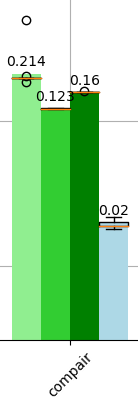
\includegraphics{afbeeldingen/outliers.png}
		\caption{Een voorbeeld van uitschieters in data van de duur van het compairprogramma.}
		\label{fig:outliers}
	\end{figure}

\section{Vormgeving resultaten}
% wat zijn de gewenste resultaten (-vormen)
	% verschillende parameters uit show_plot(): log, boxplot, normalise
	% Hoe simpeler hoe beter
In deze sectie wordt er besproken uit welke grootheden de resultaten zullen bestaan, hoe deze gevormd worden en op welke manier de resultaten gevisualiseerd worden. 

	\subsection{Gebruikte grootheden} \label{subsec:gebruiktegrootheden}
	De belangrijkste te onderzoeken parameter is de tijd. De duur van uitvoeren van een programma kan een grote factor spelen bij het maken van een kosten-baten analyse. Echter als er enkel de latency met elkaar vergeleken wordt, kan dit leiden tot een vertekend beeld. Daarom worden ook factoren zoals \gls{cpu}-gebruik en kloksnelheid in rekening gebracht. De latency per percentage \gls{cpu}-gebruik en per MHz kloksnelheid geeft een beter beeld van de performantie van elk toestel. Een andere variabele die in rekening gebracht kan worden is het vermogen dat elk toestel verbruikt. Door de latency te vermenigvuldigen met het vermogen bekomt men de energie die verbruikt wordt tijdens de executie. Voor de grootheden geldt:
	
	\begin{equation}\label{eq:power}
		time \cdot power = s \cdot \frac{J}{s} = J = Energy	
	\end{equation}
	
	Het is interessant om de verbruikte energie van de verschillende toestellen voor hetzelfde programma met elkaar te vergelijken. Toepassingen die energie gebonden zijn of waar een batterij de voeding voorziet kunnen een afweging maken tussen het energieverbruik en de duur van executie.	\\

	\subsection{Weergave resultaten}
	De weergave van de resultaten zal op een visuele wijze in een \textit{bar chart} gepresenteerd worden. Dit laat op eenvoudige wijze toe de verschillende boards te vergelijken. Dit wordt eveneens naast de tabelvorm regelmatig in de literatuur gebruikt. Enkel het omzetten naar een bar chart zal nog niet voldoende zijn om op een eenvoudige wijze vergelijkingen te maken. De resultaten voor verschillende programma's kunnen meerdere decades verschillen in grootte door gebruik van grotere datasets of complexere modellen. Bijgevolg zullen relatieve verschillen in grootte bij kleinere resultaten minder opvallen. Een manier om dit tegen te gaan is het gebruik van een logaritmische schaal voor de tijd-as. De resultaten die kleiner in grootte zijn, zullen hier beter gerepresenteerd worden. Een nadeel is wel dat de relatieve groottes tussen devices minder goed af te lezen valt. Als de lengte van een staaf van een eerste device twee maal groter is dan een tweede device betekent dit bijvoorbeeld niet dat het eerste device twee keer trager is dan de tweede. Een tweede methode die gebruikt wordt om vergelijkingen te vereenvoudigen, is het normaliseren van de data naar \'e\'en toestel toe. Dit is het herschalen van data zodat de relatieve grootte t.o.v. een vast device gepresenteerd wordt. Er worden bijvoorbeeld dus geen werkelijke latency-waarden weergegeven maar het relatieve grootteverschillen tussen een toestel en het gekozen vaste toestel. In deze thesis werd de Personal Computer als vast toestel gekozen. Door het enige non-edge toestel te gebruiken als referentiepunt kunnen vergelijkingen tussen edge toestellen zelf en tussen edge en non-edge devices beter plaats vinden. Tot slot is er ook nog de optie aanwezig om een boxplot te tonen bovenop de figuur zelf. Indien gewenst kan de spreiding van de gebruikte data gevisualiseerd worden. Deze spreiding is typisch klein genoeg zodat deze de eenvoud van de grafiek kan belemmeren. Voor deze reden is er gekozen om boxplot als optie toe te voegen, zoals in sectie \ref{sec:plotresultscode} verder uitgelegd zal worden. 
	
\section{Overzicht code} \label{sec:plotresultscode}
% Uitleg code plot results
In deze sectie wordt de gebruikte code uitgelegd. Hoe de data verkregen uit vorig hoofdstuk verwerkt wordt en hoe deze vervolgens gevisualiseerd worden. De resultaten die hier uit leiden zullen in hoofdstuk \ref{ch:resultaten} geanalyseerd en besproken worden. 

	\subsection{Ophalen data}
	In vorig hoofdstuk werd de data gemeten tijdens het uitvoeren van het programma en vervolgens opgeslagen in CSV-bestanden. Deze zullen nu opnieuw ingelezen worden. Om de juiste bestanden op te kunnen halen wordt er eerst voor elk toestel een string aangemaakt met als inhoud de overeenstemmende titel van het databestand. De vier strings worden in een lijst opgeslagen zoals in listing \ref{lst:bestandsnamen}. Eveneens worden er twee lijsten aangemaakt waar de tijds- en \gls{cpu}-data in opgeslagen wordt.
	
	\begin{lstlisting}[caption={Bijhouden van databestandsnamen voor elk toestel.},captionpos=b, label = {lst:bestandsnamen}]
# De extentie '.csv' wordt later achteraan toegevoegd
name_PC = "Benchmark_PC_Thu_Apr_2_22_05_01_2020"
name_PI = "Benchmark_PI_Fri_Apr_3_02_32_27_2020"
name_NANO = "Benchmark_NANO_Fri_Apr_3_02_11_17_2020"
name_CORAL = "Benchmark_CORAL_Wed_Apr_3_20_08_16_2020"

file_names = [name_PC, name_PI, name_NANO, name_CORAL]
data_time = [[], [], [], []]
data_CPU = [[], [], [], []]
\end{lstlisting}	
		
	De lijst met opgeslagen bestandsnamen staat toe om met behulp van for-loops de data voor elk bestand sequentieel uit de bestanden te halen. Dit wordt in listing \ref{lst:extractiedata} getoond. Hier wordt er gestart met een for-loop om elk toestel te itereren. Er worden twee tijdelijke lijsten aangemaakt: $temp1$ en $temp2$. In elk van deze lijsten komt de sequenti\"ele data van \'e\'en van de features die in vorig hoofdstuk gemeten werd. In $temp2$ wordt de tijd-data van alle iteraties en alle programma's achter elkaar toegevoegd. Analoog voor $temp1$ en het \gls{cpu}-percentage. De percentages worden wel nog omgezet naar een getal tussen nul en \'e\'en door te delen door 100. In de volgende for-lus, die alle programma's af loopt, zal de data behorende tot het huidige programma in lijstvorm toegevoegd worden. Data met betrekking to de \gls{cpu} wordt in $data\_CPU$ bijgehouden. Analoog voor tijdsdata en $data\_time$. Tot slot wordt ook de gegevens voor het totaal aan de lijst toegevoegd. Deze gegevens bestaan in het bestand maar uit \'e\'en lijn. De totale duur en de \gls{cpu}-gebruik in idle-stand werden maar \'e\'en maal uitgeschreven naar het \gls{csv}-bestand. Om eenvoud in verdere behandeling van data te behouden wordt deze data meerdere keren aan de gepaste lijst $data\_CPU$ of $data\_time$ toegevoegd. Het aantal keer dat dit gebeurd is gelijk aan het aantal iteraties, hier dus 20.
 
 	\newpage
 
	\begin{lstlisting}[caption={Ophalen data uit bestand voor elk toestel.},captionpos=b, label = {lst:extractiedata}]
# Data extraction
for device in range(len(file_names)):
	temp1, temp2, = [], []
	
	with open('./logging/' + file_names[device] + ".csv", mode='r') as results_file:
		results_reader = csv.DictReader(results_file)
		for row in results_reader:
			temp2.append(float(row['timediff']))
			temp1.append(float(row['CPU Percentage']) / 100)
	
	for program in range(len(programs)):
		data_CPU[device].append(temp1[program * iterations:((program + 1) * iterations)])
		data_time[device].append(temp2[program * iterations:((program + 1) * iterations)])
	data_CPU[device].append([])
	data_time[device].append([])
	
	for iteration in range(iterations):
		data_CPU[device][-1].append(temp1[-1])
		data_time[device][-1].append(temp2[-1])
\end{lstlisting}	
	
	Indien het ophalen van de data is afgerond, hebben de variabelen $data\_CPU$ of $data\_time$ de vorm $(4,11,20)$ oftewel een lijst met drie lagen. Voor de eerste laag bestaat bijvoorbeeld de lijst $data\_time$ uit vier elementen die elk de data voor een bepaald toestel bevatten. Elke element bevat de tweede laag. De tweede laag is een lijst op zichzelf met elf elementen. Deze elementen vertegenwoordigen de tien verschillende programma's aangevuld met het totaal van de benchmark. Elk programma bevat de volgende laag. De derde laag is een lijst met 20 elementen. Deze lijst bestaat uit de fysieke datawaarden uit de benchmark. De lengte van deze lijst is bijgevolg gelijk aan het aantal iteraties die uitgevoerd werden tijdens de benchmark. In figuur \ref{fig:vormvariabele} wordt deze structuur verduidelijkt. De structuur lijkt op het eerste zicht een ingewikkelde vorm te zijn, maar deze vorm maakt het aanspreken van specifieke datawaarden eenvoudig.
				
	\begin{figure}
		\centering
		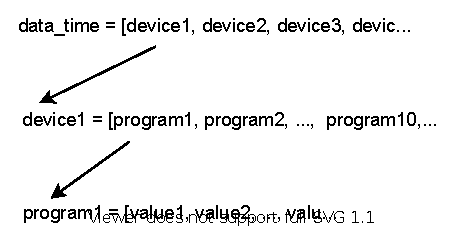
\includegraphics{afbeeldingen/shapevariable1.eps}
		\caption{De vorm van gebruikte variabelen. NOG OM TE ZETTEN NAAR VECTOR}
		\label{fig:vormvariabele}
	\end{figure}
	
	Als de data uit de benchmark is ingeladen kan het laatste deel van de benodigde data opgeslagen worden in variabelen. Deze datawaarden zijn specificatiewaarden die terug te vinden zijn in tabel \ref{tab:specdevices}. Deze worden in de vorm van lijsten opgeslagen waarbij de positie in de lijst overeenkomt met het device. De lijsten zijn in listing \ref{lst:dataspecs} weergegeven. Het betreft specificaties zoals de kloksnelheid, aankoopprijs en verbruikt vermogen. De volgende stap is het verwerken van de data.
	
	\newpage
	
		\begin{lstlisting}[caption={Data uit de specificaties voor elk toestel.},captionpos=b, label = {lst:dataspecs}]
devices = ["PC", "PI", "NANO", "CORAL"]
clockspeed = [3.25, 1.2, 1.479, 1.5]
device_price = [981, 41.5, 99, 149.99]
power = [79.9, 3.7, 5, 2.65]
\end{lstlisting}	

	\subsection{Verwerken data}
	% verwerken van data voor time/MHz/cpu%, time* power , time X price
	
	Zoals al aangegeven in subsectie \ref{subsec:gebruiktegrootheden} is het interessant om naast de latency-data ook naar grootheden zoals de duur per percentage \gls{cpu}-gebruik per MHz kloksnelheid en de verbruikte energie te kijken. Om deze grootheden te visualiseren moet er eerst op de oorspronkelijke data $data\_time$ nog enkele bewerkingen gebeuren. Deze worden in listing \ref{lst:data-time-MHzCPU} weer gegeven. In dit code-extract wordt met behulp van de for-lussen elke datawaarde opgeroepen, verwerkt en opgeslagen in de variabele $data\_time\_MHzCPU$. Hierbij is de variabele $labels\_time$ een lijst met de namen van alle programma's plus het totaal. De lengte van deze lijst die met behulp van het $len()$-commando wordt opgevraagd is dus gelijk aan het aantal elementen in de tweede laag van de variabele $data\_time$. 

		\begin{lstlisting}[caption={Verwerking van data\_time naar data\_time\_MHzCPU.},captionpos=b, label = {lst:data-time-MHzCPU}]
for device in range(len(devices)):
	for program in range(len(labels_time)):
		for iteration in range(iterations):
			data_time_MHzCPU[device][program][iteration] = data_time[device][program][iteration] / clockspeed[device] / mean(data_CPU[device][program])
\end{lstlisting}	
	
	De verwerking van $data\_time$ om de verbruikte energie te bekomen werkt analoog aan listing \ref{lst:data-time-MHzCPU} met het verschil dat elke datawaarde vermenigvuldigd wordt met het vermogen van het betreffende toestel zoals in vergelijking \ref{eq:power}.
	
	% normaliseren van data
	
	Het normaliseren van data is de volgende stap in het verwerken van de data. Met normaliseren wordt het vergelijken t.o.v. hetzelfde toestel bedoeld. Dit is een grote hulp bij het vereenvoudigen van de grafieken en bijgevolg een belangrijk onderdeel van de benchmark. In listing \ref{lst:normalisatie} kan de normalisatie verwerking gevonden worden. Aangezien er gekozen werd om met de Personal Computer te vergelijken, wordt er eerst een lijst $pc\_values$ aangemaakt. Aan deze lijst worden de gemiddelde datawaarden van de Personal Computer (dit is de index 0 in $data\_energy[0][label]$) voor elk programma toegevoegd. Vervolgens wordt elk datapunt voor elk programma in $data\_energy$ gedeeld door de corresponderende programmawaarde in $pc\_values$. Het resultaat is een lijst met drie lagen genaamd $data\_energy\_norm$. Deze bevat voor de Personal Computer waarden rond de \'e\'en met als gemiddelde voor elk programma exact \'e\'en. Voor de andere devices bevat elke datawaarde nu de relatieve grootte t.o.v. het gemiddelde van de Personal Computer.
	
	\newpage
	
		\begin{lstlisting}[caption={Normalisatie van data\_energy.},captionpos=b, label = {lst:normalisatie}]
pc_values = []
for label in range(len(labels_time)):
	pc_values.append(mean(data_energy[0][label]))

for device in range(len(devices)):
	for program in range(len(labels_time)):
		for iteration in range(iterations):
			data_energy_norm[device][program][iteration] = data_energy[device][program][iteration] \ pc_values[program]
\end{lstlisting}	

	\subsection{Visualiseren data}
	% uitleg show_plot
 	
 	De volgende stap is het visualiseren van de data. Om dit te verwezenlijken werd de hulpfunctie $show\_plot()$ aangemaakt. Deze functie wordt opgeroepen na het verwerken van de data en geeft een staafdiagram weer, waarop de data gevisualiseerd wordt. In listing \ref{lst:showplot} kan de pseudocode van de functie gevonden worden. De volledige code kan in bijlage \ref{sec:bijlageplotresults} gevonden worden. De functie beschikt over heel wat parameters die meegegeven kunnen worden. Deze worden hieronder besproken.
 	
 	\begin{itemize}
 		\item \textbf{data:} Dit is de parameter die de lijst met drie lagen bevat. Er wordt verondersteld dat de vorm voldoet aan de hierboven beschreven vorm. Deze data wordt in het programma aangepast door het gemiddelde te nemen van de waarden in de onderste laag, deze waarden af te ronden tot op 3 cijfers na de komma en vervolgens op te slaan in een nieuwe variabele $data\_bar$. De nieuwe variabele beschikt dus over maar 2 lagen met groottes $(4,11)$ of m.a.w. een matrix van 4x11.
 		\item \textbf{ylabel:} Ylabel bevat het label dat aan de y-as wordt toegekend bij het tonen van de grafiek. 
 		\item \textbf{titel:} Deze string bevat de titel die bovenaan de grafiek wordt weergegeven.
 		\item \textbf{labels:} Deze lijst van strings bevat de labels die onder aan de grafiek worden weergegeven. Deze zijn de namen van de programma's aangevuld met `total' of met `no operations' afhankelijk van het doel van de grafiek.
 		\item \textbf{log:} Deze boolean bepaalt of de y-as al dan niet in logaritmische schaal wordt gezet. Deze staat standaard op \textit{True}. Enkel bij het tonen van het \gls{cpu}-verbruik staat deze op \textit{False}.
 		\item \textbf{show:} Deze boolean bepaalt of de grafiek al dan niet getoond wordt. Deze parameter aan of uitzetten vereenvoudigt het debuggen van de code.
 		\item \textbf{index:} Deze integer houdt de volgorde van de grafieken bij. Dit wordt vooral gebruikt bij het opslaan van de grafieken volgens een unieke naam.
 		\item \textbf{boxplot:} Deze boolean bepaalt of er bovenop de staafdiagrammen de gepaste boxplots geplaatst moeten worden. 
 		\item \textbf{normalise:} Deze boolean bepaalt of de meegegeven data op een speciale wijze wordt weergegeven of niet. Wordt de data niet genormaliseerd, dan worden alle vier de devices naast elkaar in staafvorm getoond. Wordt de data wel genormaliseerd zullen enkel de edge-devices in staafvorm gepresenteerd worden en zal de Personal Computer getoond worden met behulp van een rode lijn. 
 	\end{itemize}
 	

 	
	\begin{lstlisting}[caption={Pseudocode van de show\_plot()-functie.},captionpos=b, label = {lst:showplot}]
def show_plot(data, ylabel, titel, labels, log, show, index, boxplot, normalise):
	if show = false: return #do nothing
		
	def autolabel(rects): # autolabelscript voor waarden boven elke staaf
		for rect in rects:
			height = rect.get_height()
			ax.annotate('{}'.format(height), xy=(rect.get_x() + rect.get_width() / 2, height), xytext=(0, 3), textcoords="offset points", ha='center', va='bottom')
	
	data_bar = [[], [], [], []]
	for device in range(len(devices)):
		for program in range(len(labels)):
			data_bar[device].append(float(round(mean(data[device][program]), 3)))

	fig, ax = plt.subplots()
	x = np.arange(len(labels))	# De x-coordinaten voor de labels.
	
	if normalise = false: # Indien er niet genormaliseerd wordt
		// Voeg de data in staafdiagram toe voor alle vier de devices
		// Autolabel elke staaf
		if boxplot:
			// Voeg boxplot toe bovenop elke staaf.
	elif normalise:
		// Voeg de data in staafdiagram toe voor de drie edge-devices
		// Autolabel elke staaf
		// Voeg rode lijn toe ter hoogte van y = 1
		if boxplot:
			// Voeg boxplot toe bovenop elke staaf.
	
	// Voeg labels, titel, legende, etc. toe in gewenste grootte, vorm, rotatie
	if log: # Zet de y-as in logaritmische schaal indien gewenst.
		plt.yscale("log") 
	plt.savefig(image_path + "Figure_{}".format(index)) # Opslaan van elke grafiek op gewenst adres volgens uniek index
	plt.show() # Plot the results
\end{lstlisting}
 
  	In listing \ref{lst:showplotvb} is een voorbeeld van gebruik weergegeven. Hierin worden alle parameters ingevuld op de figuur met de duur uitgedrukt per \gls{cpu}-percent per MHz. In totaal zal deze functie zeven keer uitgevoerd worden en zullen we dus zeven staafdiagrammen krijgen.  
 
	\begin{lstlisting}[caption={Voorbeeld van gebruik van de show\_plot()-functie.},captionpos=b, label = {lst:showplotvb}]
show_plot(data_time_MHzCPU_norm,
			ylabel="Time / CPU% / MHz.",
			titel="Time / CPU% / MHz for each device, Normalised.",
			labels=labels_time,
			log=True, show=False, index=4,
			boxplot=False, normalise=True)
\end{lstlisting}	
 	
 	
 	% visualiseren via tabel
 	
 	% benchmark is makkelijk uitbreidbaar


